%----------------------------------------------------------------------------------------
%
% LaTeX-template for degree projects at LNU, Department of Computer Science
% Last updated by Johan Hagelbäck, Oct 2015
% Linnaeus University
%
% License: Creative Commons BY
%
%----------------------------------------------------------------------------------------

%----------------------------------------------------------------------------------------
%	Settings and configuration
%----------------------------------------------------------------------------------------

\documentclass[a4paper,12pt]{article}

\usepackage[T1]{fontenc}
\usepackage{times}
\usepackage[english]{babel}
\usepackage[utf8]{inputenc}
\usepackage{wallpaper}
\usepackage[absolute]{textpos}
\usepackage[top=2cm, bottom=2.5cm, left=3cm, right=3cm]{geometry}
\usepackage{appendix}
\usepackage[nottoc]{tocbibind}
\usepackage{enumerate}
\usepackage{array}
\newcolumntype{L}[1]{>{\raggedright\let\newline\\\arraybackslash\hspace{0pt}}m{#1}}

\setcounter{secnumdepth}{3}
\setcounter{tocdepth}{3}

\usepackage{sectsty}
\sectionfont{\fontsize{14}{15}\selectfont}
\subsectionfont{\fontsize{12}{15}\selectfont}
\subsubsectionfont{\fontsize{12}{15}\selectfont}
\usepackage[font=large, labelfont=bf]{caption}

\usepackage{csquotes} % Used to handle citations

\renewcommand{\thetable}{\arabic{section}.\arabic{table}}  
\renewcommand{\thefigure}{\arabic{section}.\arabic{figure}} 

%----------------------------------------------------------------------------------------
%	
%----------------------------------------------------------------------------------------
\newsavebox{\mybox}
\newlength{\mydepth}
\newlength{\myheight}

\newenvironment{sidebar}%
{\begin{lrbox}{\mybox}\begin{minipage}{\textwidth}}%
{\end{minipage}\end{lrbox}%
 \settodepth{\mydepth}{\usebox{\mybox}}%
 \settoheight{\myheight}{\usebox{\mybox}}%
 \addtolength{\myheight}{\mydepth}%
 \noindent\makebox[0pt]{\hspace{-20pt}\rule[-\mydepth]{1pt}{\myheight}}%
 \usebox{\mybox}}

%----------------------------------------------------------------------------------------
%	Title section
%----------------------------------------------------------------------------------------
\newcommand\BackgroundPic{
    \put(-2,-3){
    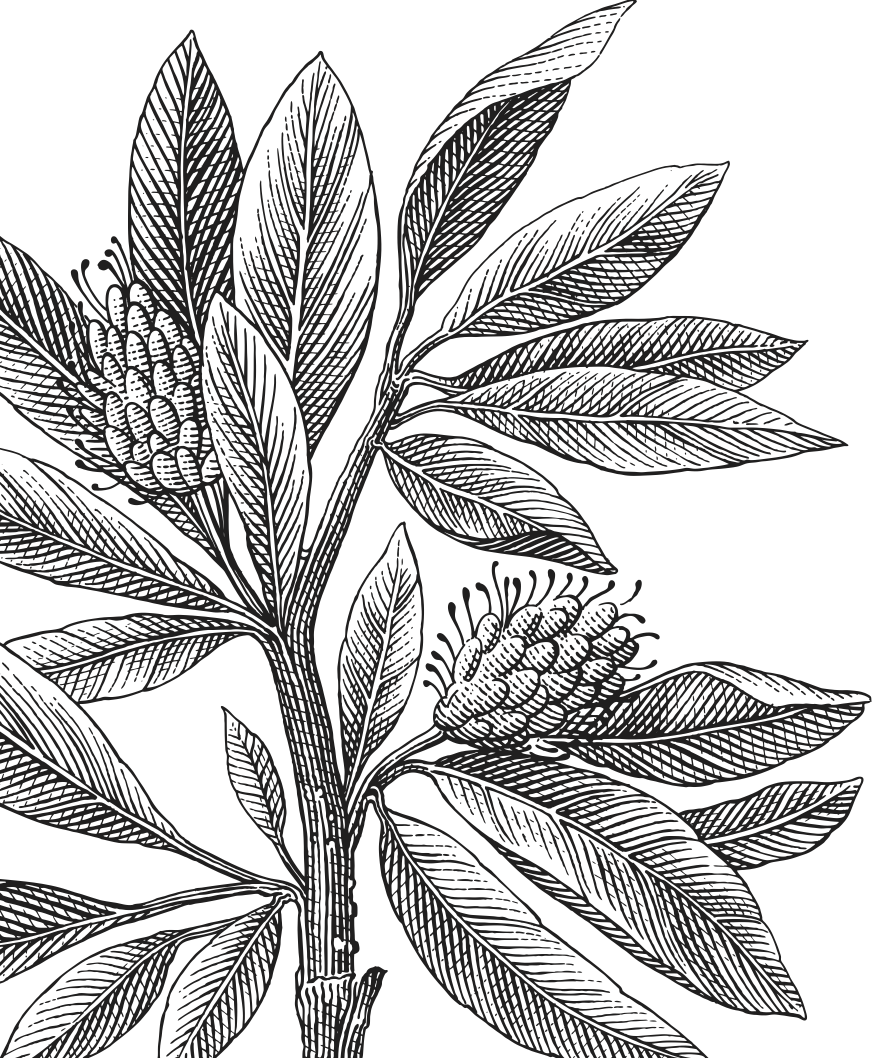
\includegraphics[keepaspectratio,scale=0.3]{img/lnu_etch.png} % Background picture
    }
}
\newcommand\BackgroundPicLogo{
    \put(30,740){
    
\includegraphics[keepaspectratio,scale=0.10]{img/logo.png} % Logo in upper left corner
    }
}

\title{	
\vspace{-8cm}
\begin{sidebar}
    \vspace{10cm}
    \normalfont \normalsize
    \Huge Report \\
    \vspace{-1.3cm}
\end{sidebar}
\vspace{3cm}
\begin{flushleft}
    \huge Project Course In Computer Science\\ 
    \it \LARGE - Deliveries Document
\end{flushleft}
\null
\vfill
\begin{textblock}{6}(10,13)
\begin{flushright}
\begin{minipage}{\textwidth}
\begin{flushleft} \large
\emph{Author:} Quasim Aljubarah, Michael Johansson, Tadas Lisauskas, Zeyuan Li, Robin Reijo and Robin Stempa\\ % Author
\emph{Supervisor:} Ola Petersson\\ % Supervisor
%\emph{Examiner:} Dr.~Mark \textsc{Brown}\\ % Examiner (course manager)
\emph{Semester:} VT 2016\\ % 
\emph{Subject:} 1DV508\\ % Subject area
\end{flushleft}
\end{minipage}
\end{flushright}
\end{textblock}
}

\date{} 

\begin{document}
\pagenumbering{gobble}
\newgeometry{left=5cm}
\AddToShipoutPicture*{\BackgroundPic}
\AddToShipoutPicture*{\BackgroundPicLogo}
\maketitle
\restoregeometry
\clearpage

\selectlanguage{english}

\tableofcontents

\newpage
\pagenumbering{gobble}
\pagenumbering{arabic}

%----------------------------------------------------------------------------------------
%
%	Here follows the actual text contents of the report.
%
%----------------------------------------------------------------------------------------
\section{Revision History}

\begin{table}[htbp]
	\centering
	\begin{tabular}{|L{4cm}|L{8cm}|L{4cm}|}
		\hline
		\textbf{Change} & \textbf{Description} & \textbf{Name and Date} \\ \hline
		Created Revision history table	&       included a revision history table to the document           &     Michael Johansson, 18/4 -2016               \\ \hline
		&                      &                        \\ \hline
	\end{tabular}
\end{table}
\newpage

\section{Introduction}
In this document we will set the start and finishing date on our different requirements from the analysis document. We will choose which requirement that should be completed when and also in what order. 

\begin{table}[htbp]
	\centering
	\caption{Deliveries}
	\label{my-label}
	\begin{tabular}{|L{4cm}|L{8cm}|L{3cm}|}
		\hline
		\textbf{Delivery and Date}& \textbf{Description and Ds}                                                                                                                                                                                                                                                                                   & \textbf{Status} \\ \hline
		\textbf{Delivery 1  20/4 - 2016} & The admin page functionality should be almost done with add product etc. \newline The database should be up and running with all the tables done and all columns. \newline IDs to be done: 1, 1.1, 1.1.1, 3, 3.1, 3.2, 3.2.1, 3.2.2                                                                   &                 \\ \hline
		\textbf{Delivery 2 27/4 - 2016} & The admin should be able to add, replace and remove categories. \newline All the categories should be defined. \newline IDs to be done: 1.1.2, 3.2.3, 3.2.4                                                                                                                                            &                 \\ \hline
		\textbf{Delivery 3 4/5 - 2016}  & The Cart should be working so the User can add, remove and change products in the cart. \newline IDs to be done: 2.2, 2.2.1, 2.2.2, 2.2.3                                                                                                                                                      &                 \\ \hline
		\textbf{Delivery 4 11/5 - 2016} & The User should be able to search, show all products in category and browse all products. \newline The User should be able to click on a product to get more info about it. \newline Admin should be able to add new and remove existing admin accounts. \newline IDs to be done: 2, 2.1, 3.3, 3.3.1          &                 \\ \hline
		\textbf{Delivery 5 18/5 - 2016} & The User should be able to place orders.\newline An Admin should be able to change and update orders. \newline The User should get an orderID when placing an order. \newline The User should be able to check his order with the orderID. \newline IDs to be done: 1.2, 1.2.1, 2.3, 2.3.1, 2.3.2, 2.3.3, 3.4, 3.4.1 &                 \\ \hline
		\textbf{Delivery 6 25/5 - 2016} & Finishing touches and CSS fine tune.                                                                                                                                                                                                                                                                                             &                 \\ \hline
	\end{tabular}
\end{table}
\newpage
\section{Conclusion}
We choose to start with the administrator pages and implementing the products. We also choose to have the sixth delivery to finishing touches and so that we have a seminar to fall back on if there is any problems along the way.

\end{document}
